\externaldocument{chapter6}
\chapter{Automated Discovery of Failure Domain Plus}
\label{chap:ADFD+}

%This paper presents Automated Discovery of Failure Domain+ (ADFD+), an upgraded version of ADFD technique with respect to algorithm and graphical presentation of failure domains. The new algorithm used in ADFD+ searches for failure domain around the failure in a given radius as against ADFD which limits the search between lower and upper bounds. This results in consumption of lower number of test cases for detecting failure domain. The output has been improved in ADFD+ to provide labelled graphs for depicting the results in easily understandable user friendly form. ADFD+ is compared with Randoop to find the comparative performance of the two techniques. The results indicate that ADFD+ is a promising technique for finding failure and failure domain efficiently and effectively. In comparison with Randoop, its efficiency is evident by taking two orders of magnitude less time and its effectiveness is shown by taking 50\% or less number of test cases to discover failure domains. ADFD+ has the added advantage of presenting the output in graphical form showing point, block and strip domains visually as against Randoop which lacks graphical user interface.




%This paper presents Automated Discovery of Failure Domain+ (ADFD+), an improvement on our previously developed Automated Discovery of Failure Domain (ADFD) technique.  ADFD+ is a random testing technique which after identifying a failure searches its surrounding to find its domain within the set range. The result obtained is graphically presented. To find the effectiveness of our Technique, several error-seeded one and two-dimensional numerical programs fwith point, block and strip failure domain were evaluated independently for 30 times by both ADFD+ and Randoop. Results indicated that ADFD+ can identify failure and failure-domain sufficiently quick and in fewer number of test cases as compared to Randoop. Additionally ADFD+ presents the failure and failure domains in a graphical form.
%\end{abstract}

%A category including the fourth, optional field follows...
%\category{D.2.5}{Software Engineering}{Metrics}[complexity measures, performance measures]

%\terms{Comparison, Verification, }
%\terms{software testing, automated random testing, ADFD}
%\begin{IEEEkeywords}
%software testing, automated random testing, ADFD.
%\end{IEEEkeywords}}


%\IEEEpeerreviewmaketitle



%%%%%%%%%%%%%%%%%    INTRODUCTION   %%%%%%%%%%%%%%%%%%%%

\section{Introduction}\label{sec:intro6}
Software testing is most widely used for verification and validation process. Efforts have been continuously made by researchers to make the testing process more and more effective and efficient. Testing is efficient when maximum number of test cases are executed in minimum possible time and it is effective when it finds the maximum number of faults in minimum number of test cases~\cite{runeson2006we}. During up-gradation and development of testing techniques, focus is always on increasing the efficiency by introducing partial or complete automation of the testing process and the effectiveness by improving the algorithm. 

%\blfootnote{Manuscript received Feb 5, 2014; revised March 20, 2013. The authors are with the Department of Computer Science, University of York, YO10 5DD, UK (e-mail: mian.ahmad@york.ac.uk, manuel.oriol@york.ac.uk).}

%Boundary Value Analysis (BVA) is one of the technique used of increasing test effectiveness. In BVA test cases with boundary values are added to the test suite with the assumption that errors reside along the boundaries~\cite{radatz1990ieee}. Daikon~\cite{ernst2007daikon} is an automatic tool used to improve the efficiency. It saves testers time by automatically generating likely program invariants.
%However, the two approaches can adversely affect the testing process if wrong boundaries or invariants are taken into consideration. It is therefore motivating to accurately identify the boundaries of the input domain in BVA and measure the degree of correctness of auto-generated invariants by Daikon in the case of point, block and strip failure domain. 


%A number of empirical evidence confirms that failure revealing test cases tend to cluster in contiguous regions across the input domain~\cite{finelli1991nasa, schneckenburger2007towards}. According to Chan et al.~\cite{chan1996proportional} the clusters are arranged in the form of point, block and strip failure domains. In the point domain the failure revealing inputs stand-alone and are evenly spread throughout the input domain. In block domain, the failure revealing inputs are contiguously clustered in one area. In strip domain, the failure revealing inputs are clustered in one long elongated strip.  %Figure~\ref{fig:patterns2} shows failure domains of the three types for two-dimensional program. 


To target failures and evaluate the failure domains we developed earlier ADFD technique \cite{ahmad2013adfd}. The ADFD$^+$, an improved version of ADFD, is a fully automatic technique which finds failures and failure domains within a specified radius and presents the results on a graphical chart. The efficiency and effectiveness of ADFD$^+$ technique is evaluated by comparing its performance with that of a mature testing tool Random tester for object-oriented programs (Randoop)~\cite{pacheco2007randoop}. The results generated by ADFD$^+$ and Randoop for the error-seeded programs shows better performance of ADFD$^+$ with respect to time and number of test cases to find failure domains. Additionally ADFD$^+$ presents the results graphically showing identified point, block and strip domains visually as against Randoop, which lacks graphical user interface.
%\begin{figure}[H]                                    
%\centering
%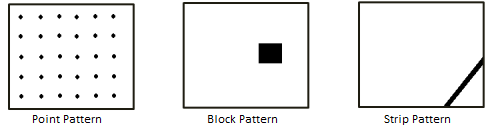
\includegraphics[width= 7cm,height=2cm]{ART_Patterns.png}
%\caption{Failure domains across input domain~\cite{chan1996proportional}}
%\label{fig:failurePatterns}
%\end{figure}
%\begin{figure} [H]
%\centering
%\subfigure[Point domain]{
%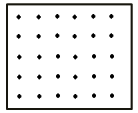
\includegraphics[width=2.5cm,height=2cm]{point.png}
%\label{fig:point}
%}
%\subfigure[Block domain]{
%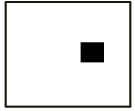
\includegraphics[width=2.5cm,height=2cm]{block.png}
%\label{fig:block}
%}
%\subfigure[Strip domain]{
%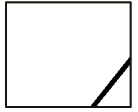
\includegraphics[width=2.5cm,height=2cm]{strip.png}
%\label{fig:strip}
%}
%\smallskip
%\caption{Failure domains across input domain~\cite{chan1996proportional}}
%\label{fig:patterns2}
%\end{figure}
%This paper describes the new ADFD+ technique developed for automatically finding failures, failure domains and graphical presentation of results. In this technique, the test execution is initiated by random+  and continues till the first failure is found in the SUT. The technique then copies the values leading to the failure and the surrounding values to the dynamic list of interesting values. The resultant list provides relevant test data for the remaining test session and the generated test cases are more targeted towards finding new failures around the existing failures in the given SUT.
%The technique uses random+ \cite{Ciupa2007, ciupa2008finding} in the initial phase. After identification of a failure, ADFD+ searches its surrounding to find its failure domain within the specified range. 


%The rest of the paper is organized as follows: Section II presents an overview of ADFD+ technique. Section III evaluates and compares ADFD+ technique with Randoop. Section IV reveals results of the experiments. Section V discusses the results. Section VI presents the threats to validity. Section VII presents related work. Finally, Section VIII concludes the study.

%The main contributions of the study are:
%\begin{itemize}
%\item \textbf{ADFD+:} It is an extension of Automated Discovery of Failure Domain (ADFD) strategy developed by Ahmad and Oriol~\cite{ahmad2013adfd}. The new technique improves the search algorithm of ADFD and makes the report more intuitive (Section \ref{sec:adfd+}).
%\item \textbf{Implementation of ADFD+:} It is implemented and intgrated in the York Extensible Testing Infrastructure \cite{Oriol2011yeti} (Section \ref{implementation_yeti}).
%\item \textbf{Evaluation:} The results generated by ADFD+ and Randoop about failure domains in the error-seeded programs are evaluated (Section \ref{evaluation}). The results show that although ADFD+ outperform Randoop with respect to time and number of test cases to find a failure domain. Additionally ADFD+ presents the results graphically. 
%\item \textbf{Future work:} ADFD+ can be extended to find and plot failure domains in multi-dimensional non-numerical programs (Section \ref{futurework}).
% A case study suggesting that boundaries are properly recognized by Daikon and ADFD+ or Daikon lake .... etc.
%\end{itemize}
%The rest of this paper is organised as follows: \\ Section~\ref{sec:adfd} describes the ADFD+ strategy. Section~\ref{sec:imp} presents implementation of the ADFD+ strategy. Section~\ref{sec:eval} explains the experimental setup. Section~\ref{sec:res} shows results of the experiments. Section~\ref{sec:discussion} discusses the results. Section~\ref{sec:rw} presents related work and Section~\ref{sec:conc}, concludes the study.


%In the later part we plot the domain on the basis of invariants generated by Daikon and compare both the domains.

%%%%%%%%%%%%%%%%%    Background   %%%%%%%%%%%%%%%%%%%

%\section{Preliminaries} \label{preliminaries}


%In Section~\ref{sec:adfd+} we describe the ADFD+ framework that can find the failure, its domain and plot the domain up to the specified range in a graphical form. Experiments confirms the successful working of ADFD+.


 

%%%%%%%%%%%%%%%%%    ADFD+   %%%%%%%%%%%%%%%%%%%

\section{Automated Discovery of Failure Domain$^+$}\label{sec:adfd+}
It is an improved version of ADFD, a technique developed earlier by Ahmad and Oriol~\cite{ahmad2013adfd}. The technique automatically finds failures, failure domains and present the results in graphical form. In this technique, the test execution is initiated by random$^+$ and continues till the first failure is found in the SUT. The technique then copies the values leading to the failure and the surrounding values to the dynamic list of interesting values. The resultant list provides relevant test data for the remaining test session and the generated test cases are effectively targeted towards finding new failures around the existing failures in the given SUT. \\*
The improvements made in ADFD$^+$ over ADFD technique are stated as follows.
\begin{itemize}
\item ADFD$^+$ generates a single Java file dynamically at run time to plot the failure domains as compared to one Java file per failure in ADFD. This saves sufficient time and makes the execution process quicker.

\item ADFD$^+$ uses (x, y) vector-series to represent failure domains as opposed to the (x, y) line-series in ADFD. The vector-series allows more flexibility and clarity to represent failure and failure domains.   

\item ADFD$^+$ takes a single value for the radius within which the strategy searches for a failure domain whereas ADFD takes two values as lower and upper bounds representing x and y-axis respectively. This results in consumption of the lower number of test cases for detecting failure domain.

\item In ADFD$^+$, the algorithm of dynamically generating Java file at run-time has been made simplified and efficient as compared to ADFD resulting in reduced overhead.

\item In ADFD$^+$, the point, block and strip failure domains generated in the output graph present a clear view of pass and fail domains with individually labelled points of failures as against a less clear view of the pass and fail domains and lack of individually labelled points in ADFD. %The points are also labelled for clarification. % as shown in Figure~\ref{fig:Workflow}. 

%The difference in representation of fault by ADFD and ADFD+ can be seen in figure .... Figure x is generated by ADFD with lower bound as ... and upper bound as ... While Figure Y is generated by ADFD+ with range ... for the same program given in appendix a. 
\end{itemize}


%%%%%%%%%%%%%%%%%%%%

\subsection{Implementation of ADFD$^+$} \label{sec:implementation6}
The ADFD$^+$ technique is also implemented in automated random testing tool YETI. As stated earlier YETI consists of three main parts including core infrastructure for extendibility, strategies section for adjustment of multiple strategies and languages section for supporting multiple languages. Both strategies and languages sections have pluggable architecture for easily incorporating new strategies and languages. 
% which is available in open-source at \url{http://code.google.com/p/yeti-test/}. A brief overview of YETI is given with the focus on parts relevant to implementation of ADFD+ strategy. \\*
%YETI is a testing tool developed in Java for automatic testing of programs using random strategies. YETI meta-model is language-agnostic which enables it to test programs written in functional, procedural and object-oriented languages. YETI consists of three main parts including core infrastructure for extendibility, strategies section for adjustment of multiple strategies and languages section for supporting multiple languages. Both strategies and languages sections have pluggable architecture for easily incorporating new strategies and languages making YETI a favourable choice for implementing ADFD+ strategy. YETI is also capable of generating test cases to reproduce the failures found during the test session. 
At the moment, there are seven different random strategies including our previously developed DSSR and ADFD strategies. ADFD$^+$ strategy is also added to the strategies section of YETI by extending the $YetiADFDStrategy$. Please see Chapter~\ref{chap:yeti_3} and Chapter~\ref{chap:ADFD} for more details about YETI and ADFD respectively.

%\bigskip
%\begin{figure}[h]
%\centering
%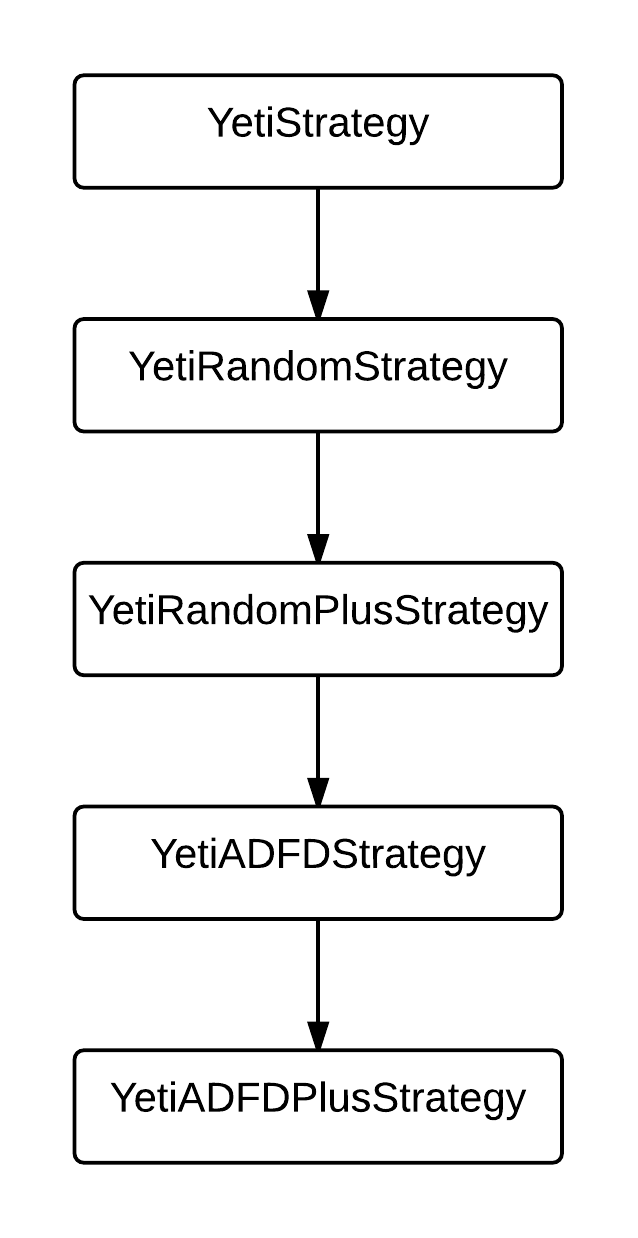
\includegraphics[width=6cm,height=9cm]{chapter6/classHierarchy3.png}
%\bigskip
%\caption{Class Hierarchy of ADFD Plus strategy in YETI}
%\label{fig:hierarchyofADFDPlus}
%\end{figure}
%\bigskip



\subsection{Workflow of ADFD$^+$} \label{sec:workflow6}
ADFD$^+$ is a fully automatic technique requiring the user to select radius value (Domain Range) and feed the program under test followed by clicking the ``Draw Fault Domain'' button for test execution. %The default range value is set to 5 meaning that ADFD+ will search 83 values around the failure. 
The work-flow of ADFD$^+$ is given in Figure~\ref{fig:Workflow6}. As soon as the button is clicked, YETI comes into play with ADFD$^+$ strategy to search for failures in the program under test. On finding a failure, the strategy creates a Java file which contains calls to the program on the failing and surrounding values within the specified radius. The Java file is executed after compilation and the results obtained are analysed to separate  pass and fail values, which are accordingly stored in the text files. At the end of test, all the values are plotted on a graph with pass values in blue and fail values in red colour as shown in Figure~\ref{fig:adfdPlusExample6}.

\bigskip
\bigskip

%Instead of front end give workflow. It will make more sense. Change the code of the program

\begin{figure}[htp]
\centering
\includegraphics[width= 13cm,height=11cm]{chapter6/adfdPlusWorkflow.png}
\bigskip
\caption{Workflow of ADFD$^+$}
\label{fig:Workflow6}
\end{figure}
\bigskip
\bigskip
%%%%%%%%%%%%%%%%%%%%
%ADFD+ is an extension of ADFD's algorithm with more accuracy to find and clarity to plot the failure domain on a graphical chart. Deriving failure domains using ADFD+ is a one click process and all the tester needs to input is the class to test and the range-value for which to search around the found failure. 
%%%%%%%%%%%%%%%%%%%%


\subsection{Example to illustrate working of ADFD$^+$}
Suppose we have the following error-seeded class under test. It is evident from the program code that a failure is generated when the value of variable $x$ ranges between 5 to 8 and the value of variable $y$ between 2 to 4.

\begin{lstlisting}
public class Error {
  public static void errorProgram (int x, int y){
    if (((x>=5)&&(x<=8))&&((y>=2)&&(y<=4)))
		 abort();		/* error */
  } 
}
\end{lstlisting}

At the beginning of the test, ADFD$^+$ strategy evaluates the given class with the help of YETI and finds the first failure at x = 6 and y = 3. Once a failure is identified ADFD$^+$ uses the surrounding values around it to find a failure domain. The radius of surrounding values is limited to the value set by the user in the $Domain~Range$ variable. When the value of $Domain~Range$ is set to 5, ADFD$^+$ evaluates a total of 83 values of $x$ and $y$ around the found failure. All evaluated $(x, y)$ values are plotted on a two-dimensional graph with red filled squares indicating fail values and blue filled circles indicating pass values. Figure~\ref{fig:adfdPlusExample6} shows that the failure domain forms a block pattern and the boundaries of the failures are $(5, 2), (5, 3),(5, 4), (6, 2), (6, 4), (7, 2), (7, 4), (8, 2), (8, 3), (8, 4)$. 

\bigskip
\begin{figure*}[h]
\centering
\centerline{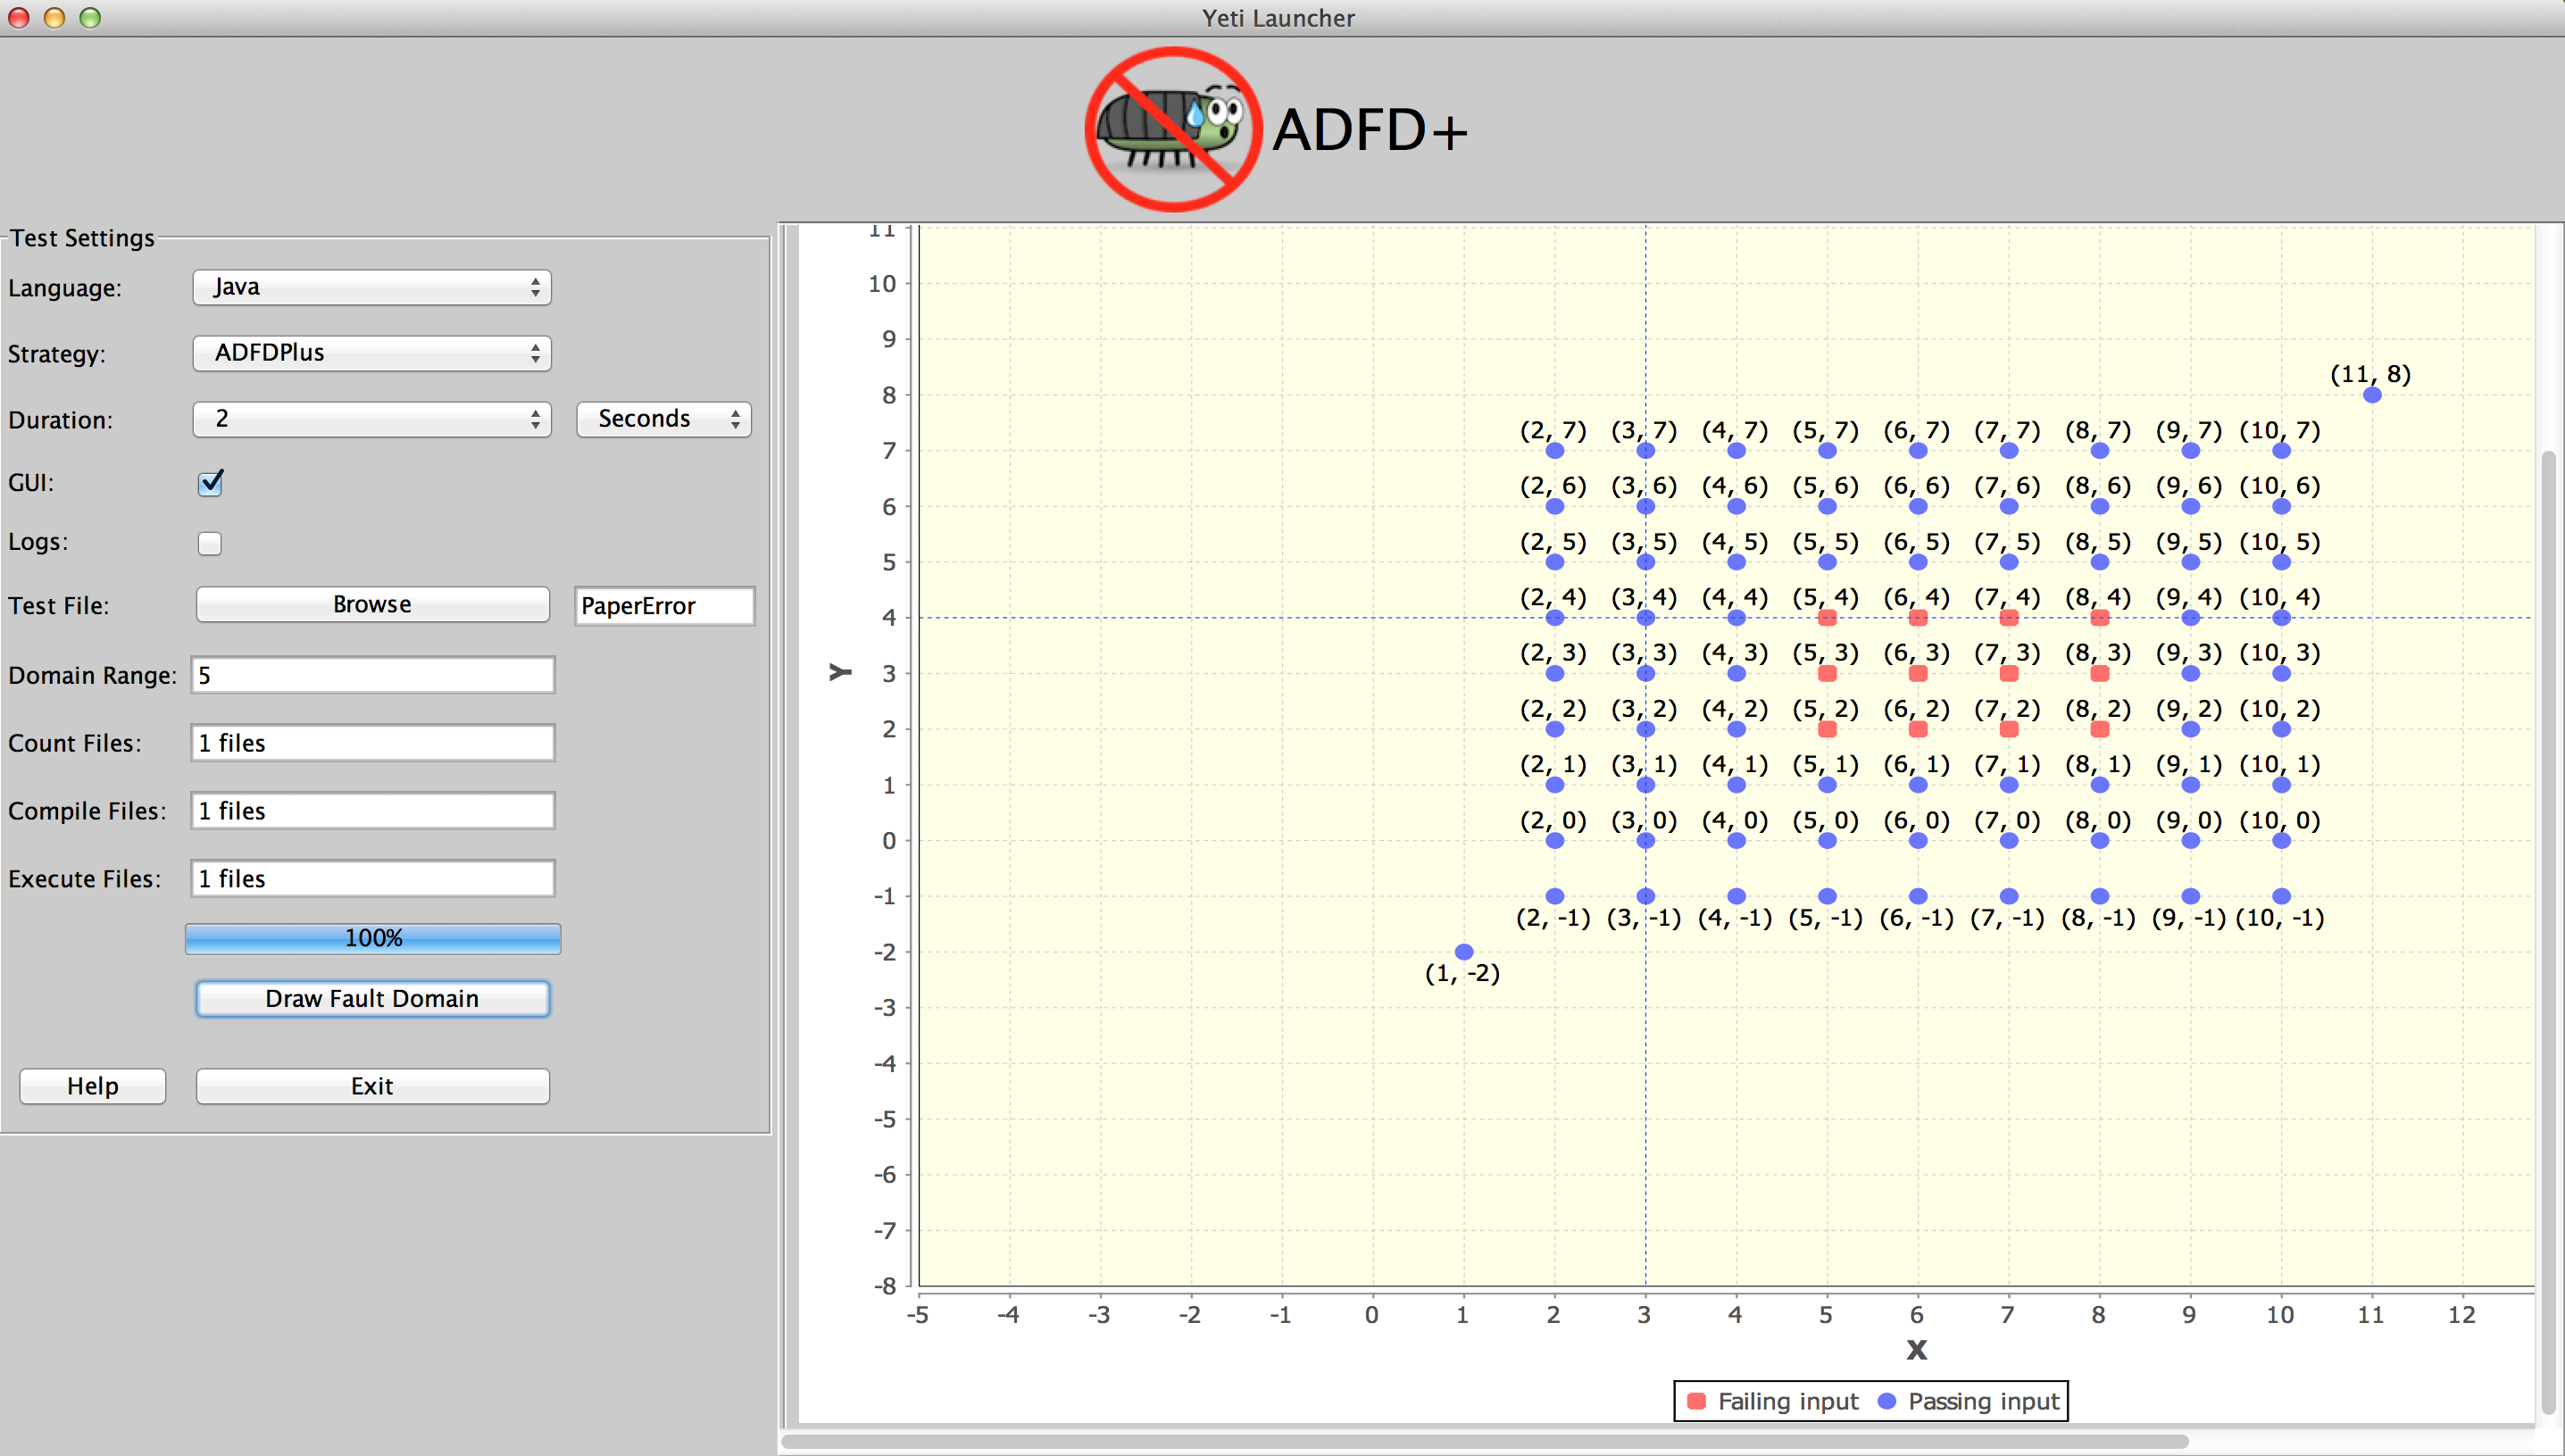
\includegraphics[width=12cm,height=8cm]{chapter6/exampleError.png}}
\bigskip
\caption{The output of ADFD$^+$ for the above code.}
\label{fig:adfdPlusExample6}
\end{figure*}
\bigskip


%%%%%%%%%%%%%%%%%%%%%%%%%%%%%%%%%%%%%%%%%%%%%%%%%



%Randoop maintains two sets called \verb+ErrorSeqs+ and \verb+NonErrorSeqs+ to record the feedback. It extends \verb+ErrorSeqs+ set in case of contract or filter violation and \verb+NonErrorSeqs+ set when no violation is recorded in the feedback. The use of this dynamic feedback evaluation at runtime brings an object to an interesting state. On test completion, \verb+ErrorSeqs+ and \verb+NonErrorSeqs+ are produced as JUnit/NUnit test suite. In terms of coverage and number of faults discovered, Randoop implementing FDRT was compared with JCrasher and JavaPathFinder and 14 libraries of both Java and .Net were evaluated~\cite{visser2004test}. The results showed that Randoop achieved more branch coverage and better fault detection than JCrasher. 



%Daikon is a tool~\cite{ernst2007daikon}, which uses machine-learning technique to automatically generate likely invariants of the program written in C, C++, Java and Pearl. Daikon takes the program and a few test cases as input. The test cases may be either generated manually or by an automated tool. Daikon executes the test cases on the program under test and observes the values that the program computes. At the end of the test session it reports the properties that were true for the observed executions. A feature of Daikon facilitate to process the generated invariants to mitigate non-interesting and redundant invariants. Another feature allows to inserts the generated invariants in to the source code as assertions. The report generated by Daikon is useful in understanding program logic, generating invariants, predicting incompatibilities in component integration, automating theorem proving, repairing inconsistencies in data structures and checking the validity of data streams.




%%%%%%%%%%%%%%%%%    EVALUATION   %%%%%%%%%%%%%%%%%%%%
%\section{Comparison of ADFD+ \& Randoop}\label{sec:eval}
%In order to check the effectiveness and efficiency of ADFD+ we compared it with a random testing tool Randoop. Our subject classes for these experiments were the same that were used in evaluation of ADFD \cite{ahmad2013adfd}. We ran ADFD+ and Randoop for 30 times on each error-seeded one and two dimensional numerical programs, measuring its effectiveness by the total number of test cases used to detect all the failures and its efficiency by the CPU time consumed. 



\section{Evaluation} \label{sec:evaluation}
For evaluating the efficiency and effectiveness, we compared ADFD$^+$ with Randoop, following the common practice of comparison of the new tool with a mature random testing tool \cite{pacheco2005eclat, oriat2005jartege, xie2005symstra}. Testing of several error-seeded one and two dimensional numerical programs was carried out as per program code \cite{ahmad2013adfd}. The programs were divided in to set A and B containing one and two-dimensional programs respectively. Each program was injected with at least one failure domain of point, block or strip nature. The failure causing values are given in Table \ref{table:failureDomains6}. Every program was tested independently for 30 times by both ADFD$^+$ and Randoop. Time taken and the number of tests executed to find all failure domains were used as criteria for efficiency and effectiveness respectively. The external parameters were kept constant in each test. Due to the absence of contracts and assertions in the code under test, undeclared exceptions were taken as failures in accordance with the previous studies~\cite{csallner2004jcrasher, oriol2012random, ducasse2011challenges}.
\bigskip

\begin{table}[h]
\caption{Table depicting values of x and y arguments forming point, block and strip failure domain in Figure \ref{fig:PFDOne6}, \ref{fig:BFDOne6}, \ref{fig:SFDOne6} and Figure \ref{fig:PFDTwo6}, \ref{fig:BFDTwo6}, \ref{fig:SFDTwo6} respectively}
\smallskip
\centering
{\renewcommand{\arraystretch}{1.3}
\begin{tabular}{|l|l|l|l|}
\hline
Dim & Point failure		& 	Block failure		& 	Strip failure		\\
\hline
One & x = -66			&	x = -1, 0, 1		&	x = -4 -- 34 	\\	
& x = -2			 	&	x =-26 -- -29	&					\\	
& x= 51 				&	x = 51 -- 54 	&					\\
& x= 23 				& 	 				& 					\\
\hline
Two &x=2, y=10			&	x = 5, y = 2		&	x = 7,~~y = 0	\\	
&x=4, y=10			&	x = 6, y = 2		&	x = 8,~~y = 0	\\	
&x=7, y=10			&	x = 7, y = 2		&	x = 8,~~y = 1	\\
&x=9, y=10			& 	x = 8, y = 2 		& 	x = 9,~~y = 1	\\
&					& 	x = 5, y = 3 		& 	x = 9,~~y = 2	\\
&					& 	x = 6, y = 3 		& 	x = 10, y = 2	\\
&					& 	x = 7, y = 3 		& 	x = 10, y = 3	\\
&					& 	x = 8, y = 3 		& 	x = 11, y = 3	\\
&					& 	x = 5, y = 4 		& 	x = 11, y = 4	\\
&					& 	x = 6, y = 4 		& 	x = 12, y = 4	\\
&					& 	x = 7, y = 4 		& 	x = 12, y = 5	\\
&					& 	x = 8, y = 4 		& 	x = 13, y = 6	\\
&					&			      		& 	x = 14, y = 6	\\				
&					&			      		& 	x = 14, y = 7	\\
\hline
\end{tabular}
}
\bigskip
\label{table:failureDomains6}
\end{table}


\newpage

\begin{figure} [htp]
\centering
\subfigure[Point failure domain in one-dimension]{
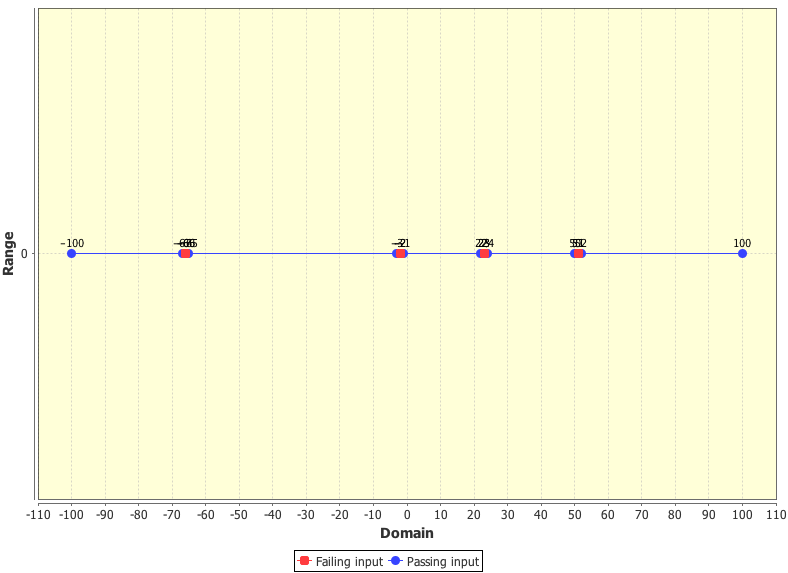
\includegraphics[width=10cm,height=6.5cm]{chapter6/PFDOne.png}
\label{fig:PFDOne6}
}
\subfigure[Block failure domain in one-dimension]{
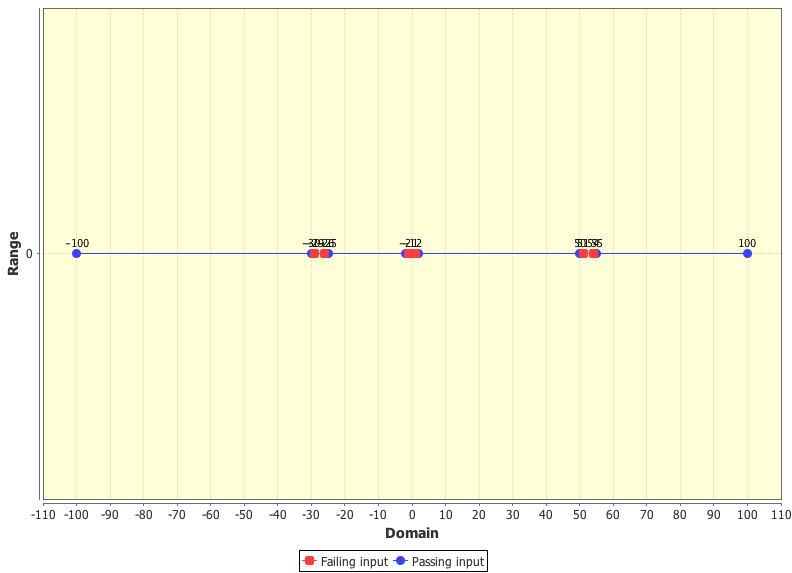
\includegraphics[width=10cm,height=6.5cm]{chapter6/BFDOne.png}
\label{fig:BFDOne6}
}
\subfigure[Strip failure domain in one dimension]{
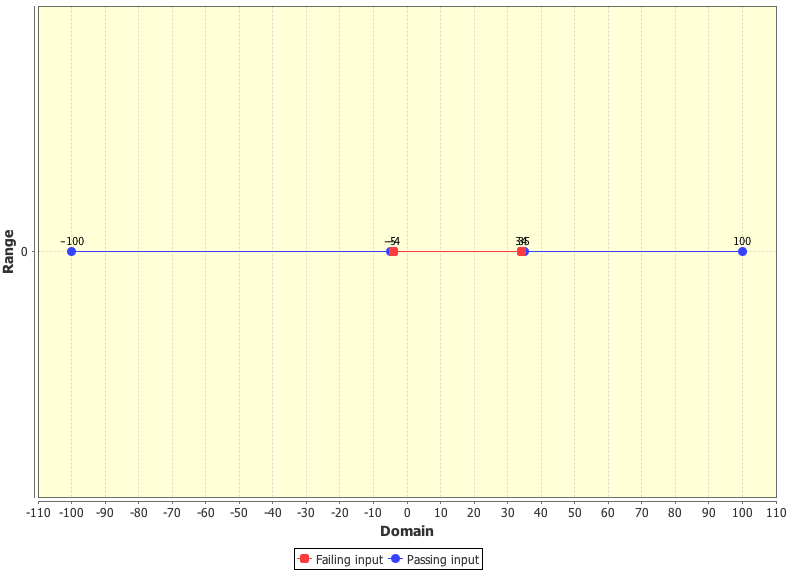
\includegraphics[width=10cm,height=6.5cm]{chapter6/SFDOne.png}
\label{fig:SFDOne6}
}
\caption{Pass and fail values plotted by ADFD$^+$ in three different cases of two-dimension programs}

\label{fig:failureDomainsOneDimension6}
\end{figure}




\begin{figure} [htp]
\centering
\subfigure[Point failure domain in two-dimension]{
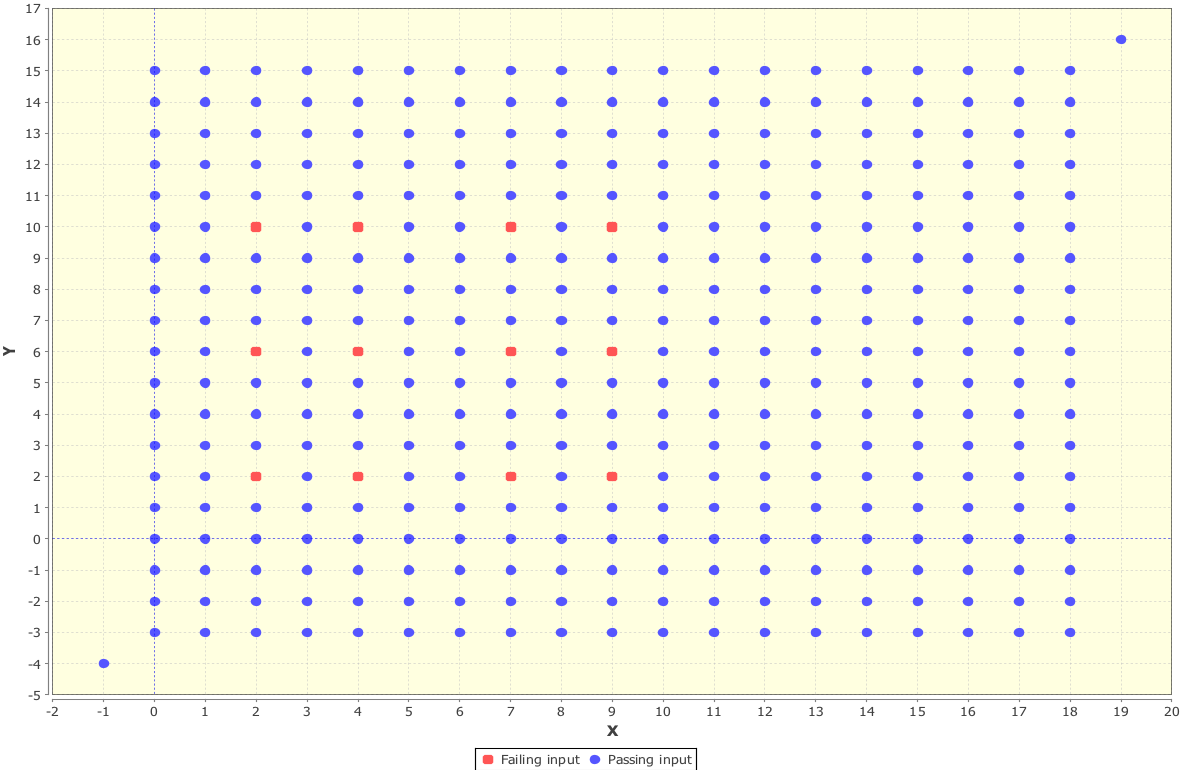
\includegraphics[width=10cm,height=6.5cm]{chapter6/PFDTwo.png}
\label{fig:PFDTwo6}
}
\subfigure[Block failure domain in two-dimension]{
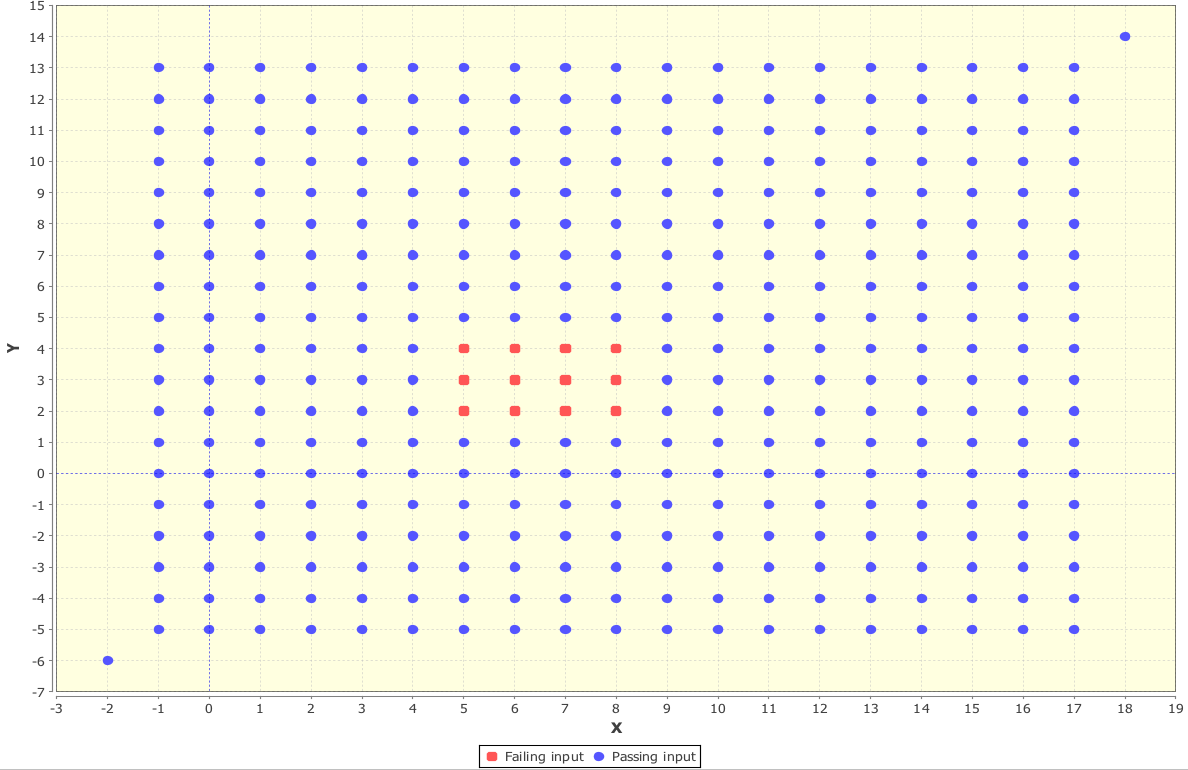
\includegraphics[width=10cm,height=6.5cm]{chapter6/BFDTwo.png}
\label{fig:BFDTwo6}
}
\subfigure[Strip failure domain in two-dimension]{
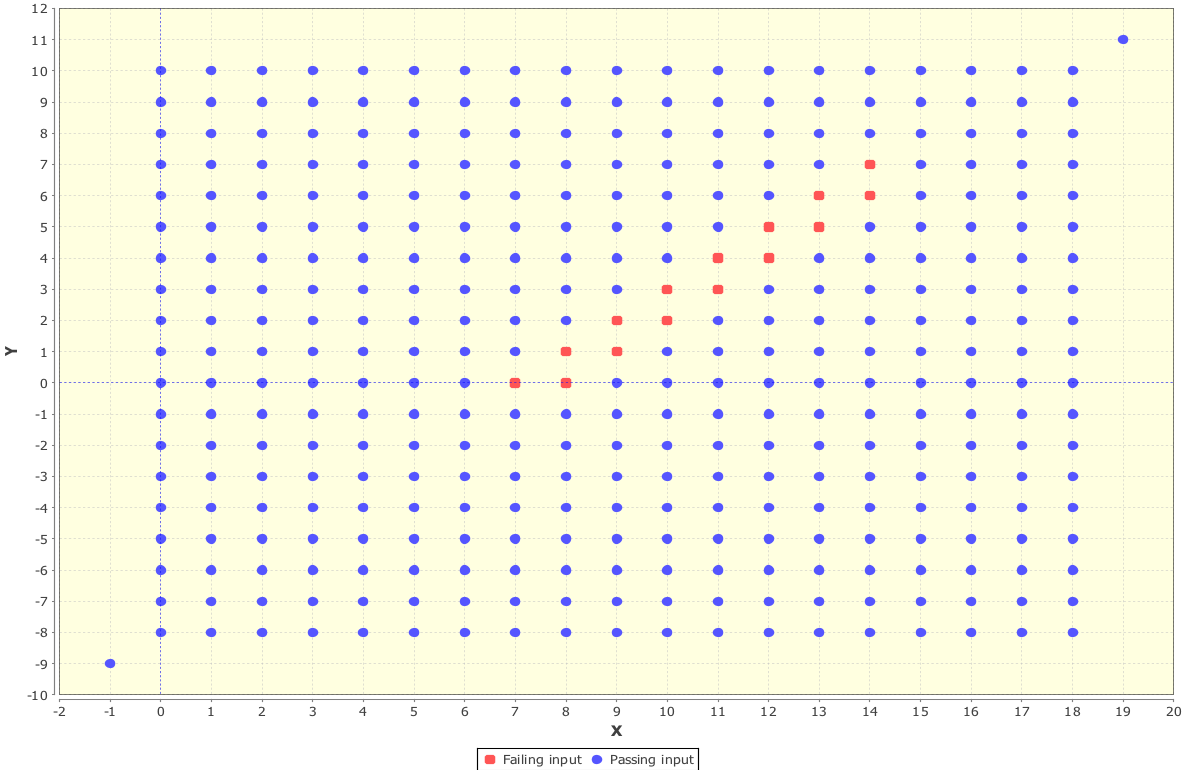
\includegraphics[width=10cm,height=6.5cm]{chapter6/SFDTwo.png}
\label{fig:SFDTwo6}
}
\caption{Pass and fail values plotted by ADFD$^+$ in three different cases of two-dimension programs}

\label{fig:failureDomainsTwoDimension6}
\end{figure}







\clearpage
\newpage
\subsection{Research questions} \label{sec:questions}
The following research questions have been addressed in the study for evaluating ADFD$^+$ technique with respect to efficiency, effectiveness and presentation of failure domains:
\begin{enumerate}
%\item \textbf{Efficiency:} How efficient is ADFD+, compared to Randoop, across different failure domains?
\item How efficient is ADFD$^+$ as compared to Randoop?
%\item \textbf{Effectiveness:} How effective is ADFD+, compared to Randoop, across different failure domains?
\item How effective is ADFD$^+$ as compared to Randoop?
%\item \textbf{Failure-domains:} How the boundaries of a failure domains are presented by ADFD+ and Randoop?
\item How failure domains are presented by ADFD$^+$ as compared to Randoop?
%5 you will also prove it through figure but you can also say ADFD+ clarify it further by showing the boundaries in graphical form.
\end{enumerate}


%Because of using error-seeded one and two dimensional numerical programs, we were aware of the failure domain present in each program. The correct identification and presentation of the failure domain by ADFD+ prove the correct working of ADFD+. We then evaluated the same program by Randoop. 













%\begin{figure}[!Htp]
%  \centering
%  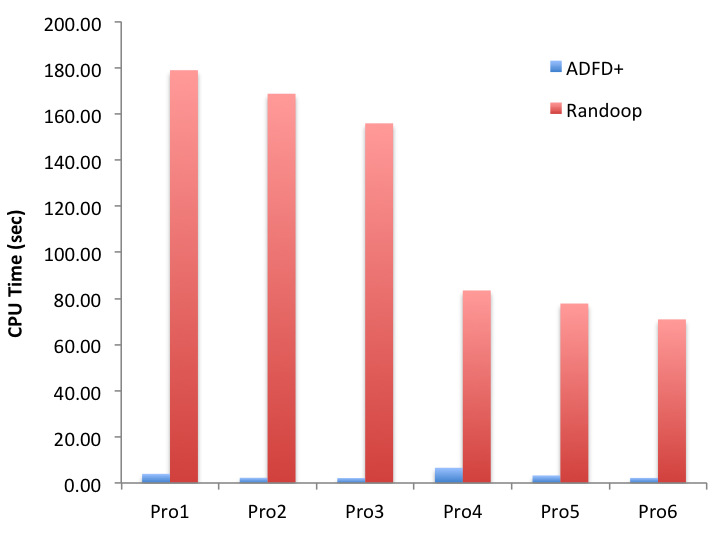
\includegraphics[width=7.5cm,height=8.5cm]{chapter6/timeTakenBar.png}
%  \caption{Time taken to find failure domains}
%  \label{fig:testtime6}
%  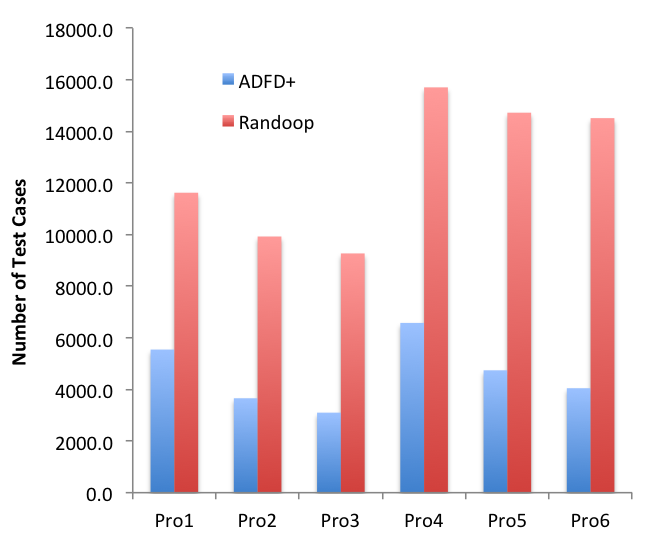
\includegraphics[width=7.5cm,height=8.5cm]{chapter6/testCasesBar.png}
%  \caption{Test cases taken to find failure domains}
%  \label{fig:testcases6}
%\end{figure}


\subsection{Randoop} \label{sec:randoop}
Random tester for object-oriented programs (Randoop) is a fully automatic tool, capable of testing Java classes and .Net binaries. It takes as input a set of classes, time limit or number of tests and optionally a set of configuration files to assist testing. Randoop checks for assertion violations, access violations and un-expected program termination in a given class. Its output is a suite of JUnit for Java and NUnit for .Net program. Each unit test in a test suite is a sequence of method calls (hereafter referred as sequence). Randoop builds the sequence incrementally by randomly selecting public methods from the class under test. Arguments for these methods are selected from the pre-defined pool in case of primitive types and as a sequence of null values in case of reference type. Randoop uses the feedback mechanism to filter out duplicate test cases. For more details about Randoop, please see Section~\ref{sec:Randoop} for more details.


%The code for the programs under test is given in Appendix~\ref{} while the test details are presented in Table~\ref{table:Results}. 
%Every class was evaluated through $10^5$ calls in each test session of ADFD+.
%\footnote{The total number of tests is equal to $60\times 30\times 3 \times 10^5 = 540\times10^6~tests$.} 
\subsection{Experimental setup}
All experiments were conducted with a 64-bit Mac OS X Mountain lion version 10.8.5 running on 2.7 GHz Intel Core i7 quad core with 16 GB (1600 MHz DDR3) of RAM. YETI runs on top of the Java\texttrademark  SE Runtime Environment [version 1.6.0\_35]. %The machine took approximately 100 hours to process the experiments.
The ADFD$^+$ Jar file is available at \url{https://code.google.com/p/yeti-test/downloads/list/} and Randoop at \url{https://randoop.googlecode.com/files/randoop.1.3.3.zip}.

The following two commands were used to run the ADFD$^+$ and Randoop respectively. Both tools were executed with default settings, however, Randoop was provided with a seed value as well.% On running command (1) the ADFD+ starts with a GUI front-end given in Figure \ref{fig:adfdPlusExample6}. On running command (2) Randoop starts in CLI mode as there is no GUI.
\begin{lstlisting}[language=bash]
$ java -jar adfd_yeti.jar -------------(1)

$ java randoop.main.Main gentests \
--testclass=OneDimPointFailDomain \
--testclass=Values --timelimit=100 ----(2)
\end{lstlisting}






\section{Experimental results} \label{sec:result6}
%The experimental results show that the ADFD+ outperformed Randoop in both the time taken and number of tests used to detect all the injected faults. The ADFD+ also provide the added benefit of presenting the results in graphical form as shown in Figure \ref{fig:failureDomainsOneDimension} and \ref{fig:failureDomainsTwoDimension}. 
%Results are split in to two sections depicting efficiency and effectiveness of the two tools.
\begin{figure}[H]
\centering
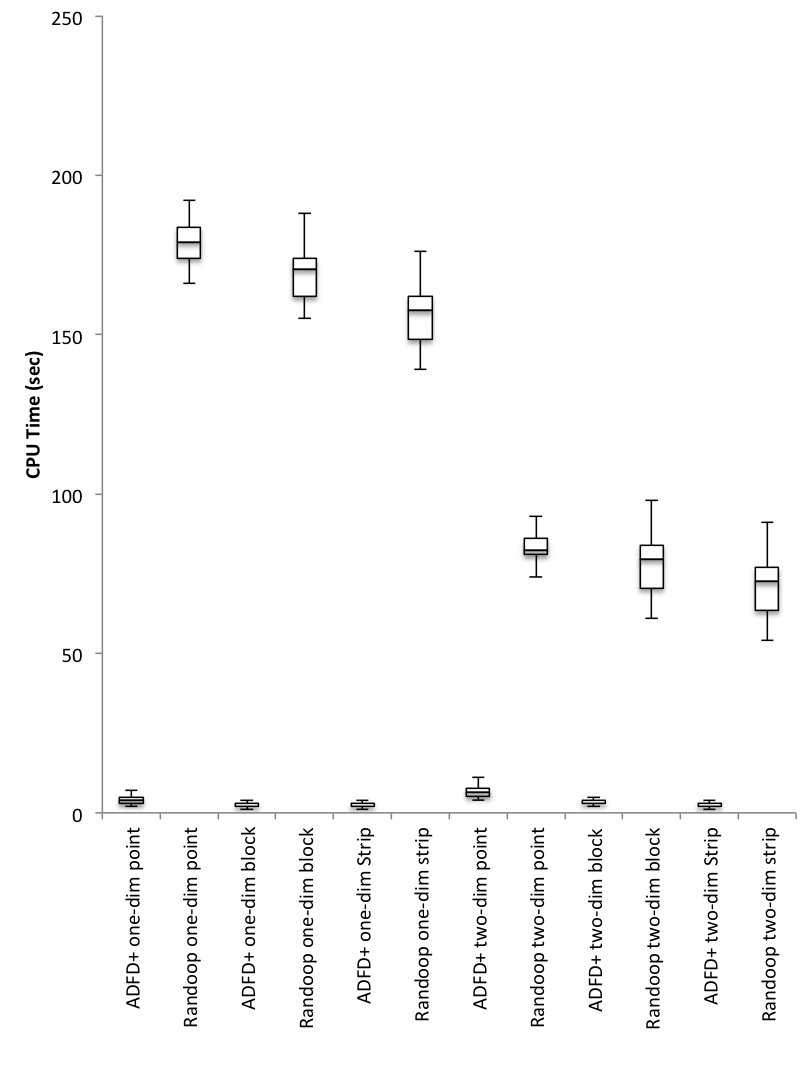
\includegraphics[width=10cm,height=9cm]{chapter6/timetaken.png}
\caption{Time taken to find failures}
\label{fig:timelimit}
\end{figure}

\begin{figure}[H]
\centering
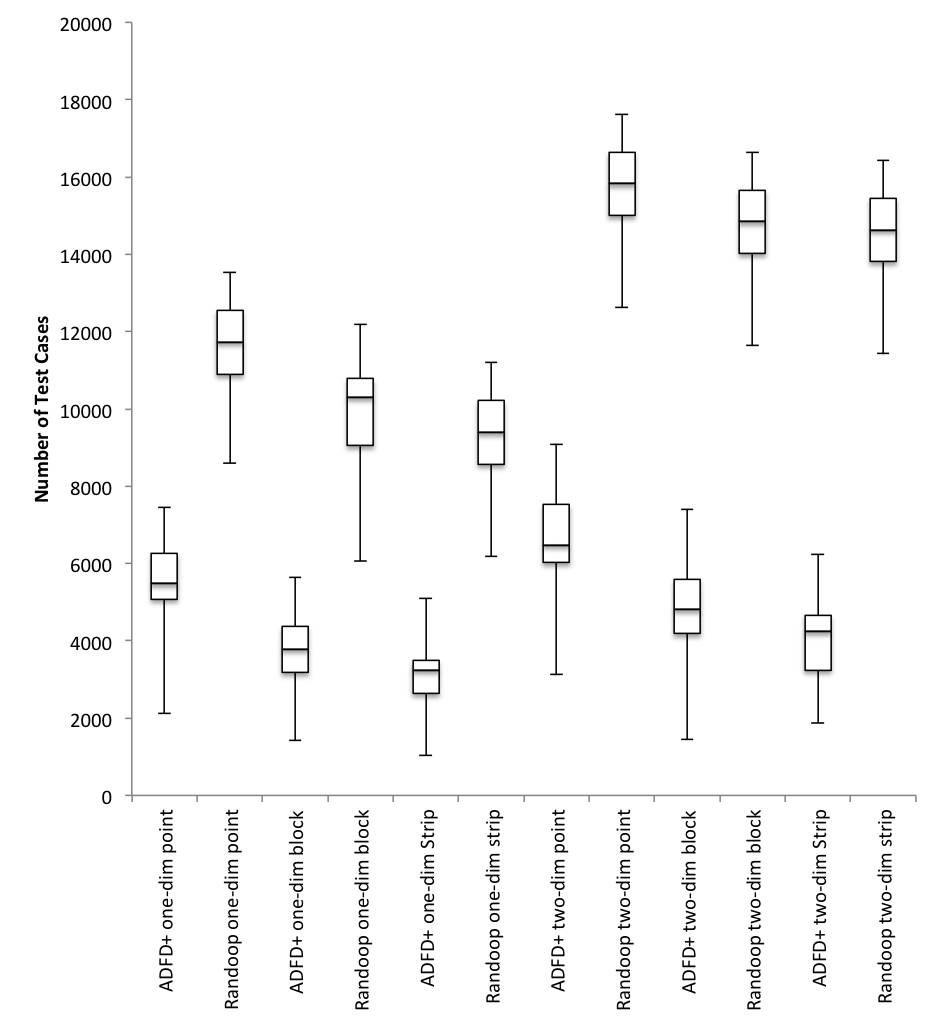
\includegraphics[width=10cm,height=9cm]{chapter6/TestCases.png}
\caption{Number of test cases taken to find failures}
\label{fig:numberoftests}
\end{figure}

\newpage
\subsection{Efficiency}
Figure \ref{fig:testtime6} shows the comparative efficiency of ADFD$^+$ and Randoop. The $x-axis$ represents one and two-dimensional programs with point, block and strip failure domains while the $y-axis$ represents the average time taken by the tools to detect the failure domains. As shown in the figure, ADFD$^+$ showed extraordinary efficiency by taking two orders of magnitude less time to discover failure domains as compared to Randoop. 

\bigskip
\begin{figure}[ht]
  \centering
  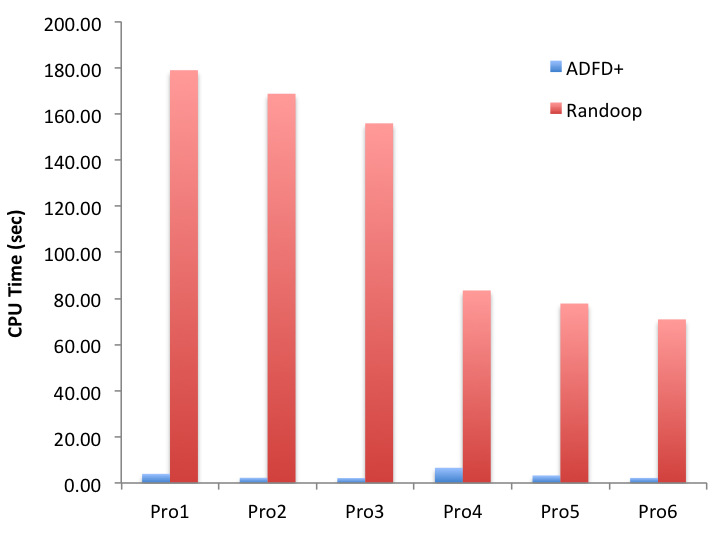
\includegraphics[width=10.5cm,height=10.5cm]{chapter6/timeTakenBar.png}
  \bigskip
  \caption{Time taken to find failure domains}
  \label{fig:testtime6}
\end{figure}
\bigskip

This may be partially attributed to the very fast processing of YETI, integrated with ADFD$^+$. YETI is capable of executing $10^6$ test calls per minute on Java code. To counter the contribution of YETI and assess the performance of ADFD$^+$ by itself, the effectiveness of ADFD$^+$ was compared with Randoop in terms of the number of test cases required to identify the failure domains without giving any consideration to the time consumed for completing the test session. The results are presented in the following section.

%It should be noted that the part of the gain may also be due to the fast processing of the underlying tool YETI, which is capable of executing $10^6$ test calls per minute on Java code. Therefore, to find the performance of only ADFD+ we performed the second set of experiments to measure effectiveness.

%For finding the efficiency, the CPU time consumed from the start of the test to the identification of last failure was measured for each experiment of ADFD+ and Randoop.  Figure \ref{fig:testtime} shows the results in a box-and-whisker plot. The figure shows that ADFD+ in no case took more than ten seconds to find the failures where Randoop consumed at least  80 seconds to find the same failures.
\subsection{Effectiveness}
Figure \ref{fig:testcases6} shows the comparative effectiveness of ADFD$^+$ and Randoop. The $x-axis$ represents one and two-dimensional programs with point, block and strip failure domains while the $y-axis$ represents average number of test cases used by the tools to detect the failure domains. The figure shows higher effectiveness in the case of ADFD$^+$, amounting to 100\% or more. The higher effectiveness of ADFD$^+$ may be attributed to its working mechanism in comparison with Randoop for identifying failures. ADFD$^+$ dynamically changes its algorithm to exhaustive testing in a specified radius around the failure as against Randoop, which uses the same random algorithm for searching failures.

\begin{figure}[ht]
  \centering
  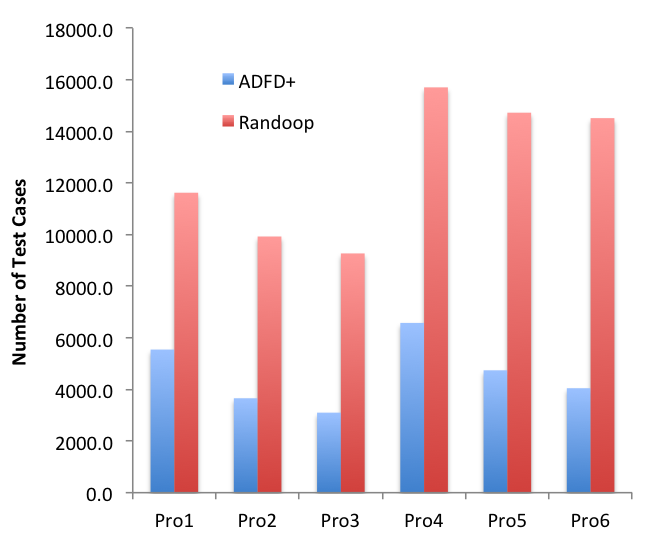
\includegraphics[width=10.5cm,height=10cm]{chapter6/testCasesBar.png}
  \bigskip
  \caption{Test cases taken to find failure domains}
  \label{fig:testcases6}
\end{figure}
\subsection{Failure Domains}
 The comparative results of the two tools with respect to presentation of the identified failure domains reveal better performance of ADFD$^+$ by providing the benefit of presenting the failure domains in graphical form as shown in Figure \ref{fig:failureDomainsOneDimension6} and \ref{fig:failureDomainsTwoDimension6}. The user can also enable or disable the option of showing the failing values on the graph. In comparison, Randoop lacks the ability of graphical presentation and the option of showing the failure domains separately. It provides the results scattered across textual files. 
 
 


%\subsubsection{Test of one-dimension programs by ADFD+}
%In each of the 30 experiments, The ADFD+ successfully discovered and plotted the failure domains for point, block and strip pattern as shown in the Figure~\ref{fig:failureDomainsOneDimension}. The lower and upper bound for each experiment are set to -100 and 100 respectively.

%\subsubsection{Test of two-dimension programs by ADFD+}
%In each of the 30 experiments, The ADFD+ once again successfully discovered and plotted the failure domain for point, block and strip failure domain as shown in the Figure~\ref{fig:failureDomainsTwoDimension}. The range value for each experiment is set to 10. Labels are disabled in the charts given in Figure~\ref{fig:failureDomainsTwoDimension} for clarity purpose. The failure values in each of the point, block and strip failure domain is given in Table~\ref{table:failureDomains}. 

%\subsection{Daikon results} \label{daikon_results}
%In initial set of experiments, Daikon failed to generate an invariant for identifying a single failure. On analysis It is found that Daikon rely on the existing set of test cases to generate invariants. Since the test cases produced by Randoop did not generate any test case from failure domain therefore Daikon could not generate an assertion to point out the failure. To enable Randoop to generate test case from failure domain we directed it to produce random values between a limited range. In this way we were able to generate interesting test cases from Randoop. Test results of Randoop are shown in Table \ref{}












%\begin{table*}[htp]
%\caption{Randoop Results}
%\centering
%{\renewcommand{\arraystretch}{1.2}
%\begin{tabular}{|l|l|r|r|r|r|r|}
%\hline
%Program	 dimension	& 	Failure domain	& 	Test time 	& Random range	& Total TC & Pass TC		& Fail TC		%\\
%\hline
%One					&	Point			&	60 sec		& -100 to 100	& 82	    & 79			& 3				%\\
%One					&	Block			&	60 sec		& -100 to 100	& 82	    & 75			& 7				%\\
%One					&	Strip			&	60 sec		& -100 to 100	& 82	    & 62			& 22			%	\\
%Two					&	Point			&	60 sec		& -100 to 100	& 6563	    & 6521		& 42			%	\\
%Two					&	Block			&	60 sec		& -100 to 100	& 5902	    & 5057		& 845			%	\\
%Two					&	Strip			&	60 sec		& -100 to 100	& 6226	    & 3896		& 2330			%	\\
%\hline
%\end{tabular}
%}
%\bigskip
%\label{table:failureDomains}
%\end{table*}


%\subsubsection{Test of one-dimensional programs by Daikon}




%\subsubsection{Test of two-dimensional programs by Daikon}





%\begin{table*}[ht]
%\caption{Table depicting values of failure points identified by ADFD+ Daikon}
%\centering
%{\renewcommand{\arraystretch}{1.3}
%\begin{tabular}{|l|l|r|r|r|r|}
%\hline
%Technique 	& Dimension	& Test cases		& 	Point failure		& 	Block failure	& 	Strip failure	\\
%\hline
%ADFD+		& 	One				& N/A			& 					& 				&				\\
%Daikon		& 	One				& 10			&					&				&				\\
%Daikon		& 	One				& 20			&					&				&				\\
%ADFD+		& 	Two				& N/A			&					&				&				\\
%Daikon		& 	Two				& 10			&					&				&				\\
%Daikon		& 	Two				& 20			&					&				&				\\
%\hline
%\end{tabular}
%}
%\bigskip
%\label{table:results}
%\end{table*}




%for point, block and strip of one dimensional program. Use the same programs of ADFD, same figures but analyse it again on Daikon. because ADFD and ADFD+ behave in the same way for one dimension. For point block and strip of two dimensional programs. Use adfd+ system.






\section{Discussion}\label{sec:discussion6}
The results indicated that ADFD$^+$ is a promising technique for finding failure and failure domain efficiently and effectively. It has the added advantage of showing the results in graphical form. The pictorial representation of failure domains facilitates the debuggers to easily identify the underlying failure domain and its boundaries for troubleshooting.

In the initial set of experiments Randoop was executed for several minutes with default settings. The results indicated no identification of failures after several executions. On analysis of the generated unit tests and Randoop's manual, it was found that the pool of values stored in Randoop database for $int$ primitive type contains only 5 values including -1, 0, 1, 10 and 100. To enable Randoop to select different values, we supplied a configuration file with the option to generate random values between -500 and 500 for the test cases as all the seeded errors were in this range. 

As revealed in the results, ADFD$^+$ outperformed Randoop by taking two orders of magnitude less time to discover the failure domains. This was partially attributed to the very fast processing of YETI integrated with ADFD$^+$. To counter the effect of YETI the comparative performance of ADFD$^+$ and Randoop was determined in terms of the number of test cases required to identify the failure domains giving no consideration to the time taken for completing the test session. As shown in the results ADFD$^+$ identified all failure domains in 50\% or less number of test cases.

The ADFD$^+$ was found quite efficient and effective in the case of block and strip domains but not so in the case of point domains where the failures lied away from each other as shown in the following code. This limitation of ADFD$^+$ may be due to the search in vain for new failures in the neighbourhood of failures found requiring the additional test cases resulting in increased overhead.
\bigskip

\begin{lstlisting}
public class ErrorClass {
  public static void errorMethod (int arg1, int arg2){
	if (arg1 == 10000) {	
		abort();		/* error */
	}	 
	if (arg2 == -20000) {	
		abort();		/* error */	
	}
  } 
}
\end{lstlisting}
\bigskip
\bigskip

%As a pilot study, we also ran an empirical study to evaluate several error-seeded programs. While it would be surprising if production programs produced much different results, it would be worthwhile to check.
The number of test cases to be undertaken in search of failures around the previous failure found is set in the range value by the user. The time taken by test session is directly proportional to the range value.  Higher range value leads to larger graphical output requiring zoom feature, which has been incorporated in ADFD$^+$ for use when the need arise.

%The implementation of ADFD+ for this pilot study has some limitations in practice, as it requires only one and two dimensional numerical programs. Though it is not difficult to extend the approach to test more than two-dimensional programs containing other primitive types, it would however be difficult to plot them on the chart as the number of coordinates increases. The approach can also be extended to test object-oriented programs by implementing objects distance proposed by Ciupa et al. \cite{ciupa2006object}. The details of such an implementation will take some effort.

\section{Threats to validity} \label{sec:threat6}
The study faces threats to external and internal validity. The external threats are common to most of the empirical evaluations. It includes the extent to which the programs under test, the generation tools and the nature of seeded errors are representative of the true practice. The present findings will serve as the foundation for future research studies needed to be undertaken with several types of classes, test generation tools and diversified nature of seeded errors in order to overcome the threats to external validity. The internal threats to validity include error-seeded and limited number of classes used in the study. These may be avoided by taking real and higher number of classes in future studies.


\section{Related Work}
The increase in complexity of programs poses new challenges to researchers for finding more efficient and effective ways of software testing with user-friendly easy to understand test results. Adaptive Random Testing \cite{chen2005adaptive}, Proportional random testing \cite{chan1996proportional} and feedback-directed random testing \cite{pacheco2007randoop} are some of the prominent upgraded versions of random testing with better performance. Automated random testing is simple to implement and capable of finding hitherto bugs in complex programs \cite{csallner2004jcrasher, pacheco2005eclat}. %ADFD+ is an upgraded version of ADFD technique \cite{ahmad2013adfd} to find a failure and using it can effectively and efficiently detect the whole failure domain.
ADFD$^+$ is a promising technique for finding failures and failure domains efficiently and effectively with the added advantage of presenting the output in graphical form showing point, block and strip domains.


Some previous research studies have reported work on Identification, classification and visualisation of pass and fail domains in the past \cite{podgurski2003automated, agrawal1995fault, jones2002visualization}. This includes Xslice~\cite{agrawal1995fault} is used to differentiate the execution slices of passing and failing part of the test in a visual form. Another tool called Tarantula uses colour coding to track the statements of a program during and after the execution of the test suite~\cite{jones2002visualization}. Hierarchical Multi Dimension Scaling (HMDS) describes a semi-automated procedure of classifying and plotting the faults \cite{podgurski2003automated}. A serious limitation of the above-mentioned tools is that they are not fully automated and require human intervention during execution. Moreover, these tools need the requirement of existing test cases to work on whereas ADFD$^+$ strategy generates test cases, discovers failures, identifies pass and fail domains and visualises the results in a graphical form operating in fully automated manner. 




\section{Summary} \label{sec:conclusion}
The newly developed ADFD$^+$ technique is distinct from other random testing techniques because it not only identifies failures but also discovers failure domains and provides the resulting output in easily understandable graphical form.  The paper highlights the improved features of ADFD$^+$ in comparison with ADFD technique previously developed by our team~\cite{ahmad2013adfd}.  The paper then analyses and compares the experimental results of ADFD$^+$ and Randoop for the point, block and strip failure domains. The ADFD$^+$ demonstrated extra ordinary efficiency  by taking less time to the tune of two orders of magnitude to discover the failure domains and it also surpassed Randoop in terms of effectiveness by identifying the failure domains in 50\% or less number of test cases.  
%The rationale for better performance of ADFD+ has been given in the paper. 
The better performance of ADFD$^+$ may be attributed mainly to its ability to dynamically change algorithm to exhaustive testing in a specified radius around the first identified failure as against Randoop which uses the same random algorithm continuously for searching failures.


%\section{Future Work} \label{sec:futurework}
%The ADFD$^+$ strategy is capable of testing numerical programs and needs to be extended for testing of non-numerical and reference data types to enable it to test all types of data.
%\textbf{Extension of ADFD+ to apply it to the real world scenario}
%The newly developed ADFD+ strategy uses error-seeded programs for assessment of accuracy and effectiveness. This may likely expose it to external validity threat.  Future studies may be undertaken in the real world scenario by including the feature of testing non numerical and reference data types so that their is more threat to validity.  \\
%Current implementation of ADFD and ADFD+ tests only numerical programs. This restricts the usability of ADFD+ for production software of non-numerical data types. This can be solved by extending the tool to include testing of other primitive and reference data types. \\
%ADFD$^+$ has the capability of graphical presentation of results for one and two-dimensional numerical programs. It is worthwhile to extend the technique to enable it to present the results of multi-dimensional numerical and non-numerical programs in a graphical form. \\

%\textbf{Introducing additional features in the user interface of ADFD+}

%The user interface of ADFD+ provides a fully automated mechanism of testing the program, processing the results and visually representing the results in graphical form. The user interface may be extended in future to give choice to the tester for real time interaction, manual addition of test cases, showing thumbnail view of previous graphs and 3D support to present multi-dimensional arguments.\\



























%%%%%%%%%%%%%%%%%    ACKNOWDLEGEMENT   %%%%%%%%%%%%%%%%%%%%
%d



%
% The following two commands are all you need in the
% initial runs of your .tex file to
% produce the bibliography for the citations in your paper.
%\bibliographystyle{abbrv}
%\bibliography{sigproc}  % sigproc.bib is the name of the Bibliography in this case
% You must have a proper ".bib" file
%  and remember to run:
% latex bibtex latex latex
% to resolve all references
%
% ACM needs 'a single self-contained file'!
%
%APPENDICES are optional
%\balancecolumns
%\bigskip

%\newpage
%\begin{wrapfigure}{l}{0.12\textwidth}
%  \vspace{-15pt}
%  \begin{center}
%    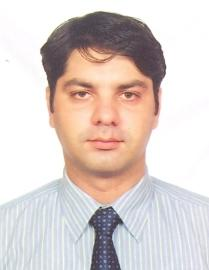
\includegraphics[width=0.13\textwidth]{mian.jpg}
%    \bigskip
%    \\
%    \bigskip
%      
\includegraphics[width=0.13\textwidth]{manuel.jpg}
%  \end{center}
%  \vspace{-20pt}
%\end{wrapfigure}
%\noindent\textbf{Mian Asbat Ahmad} is a PhD scholar at the Department of Computer Science, the University of York, UK. He completed his M(IT) and MS(CS) from Agric. University Peshawar, Pakistan in 2004 and 2009 respectively. His research interests include new automated random software testing strategies.


%\bigskip
%\noindent\textbf{Manuel Oriol} is a lecturer at the Department of Computer Science, the University of York, UK. He completed his PhD from University of Geneva and an MSc from ENSEEIHT in Toulouse, France. His research interests include software testing, software engineering, middleware, dynamic software updates, software architecture and real-time systems.

%\bigskip
%\bigskip








































\begin{comment}

%%%%%%%%%%%%%%%%%%%%%%%%%%%%%%%%%%%%%%%%%%%%%%%%%%%%%%%%%%%%%%%%%%%%%%%%%%%%%%%%%%%%%%%%%%%%%%
\scriptsize
\textbf{Program 2} Point domain with One argument
\begin{lstlisting} 
/**
 * Point Fault Domain example for one argument
 * @author (Mian and Manuel)
 */
public class PointDomainOneArgument{

	public static void pointErrors (int x){
		if (x == -66 )
			x = 5/0;

		if (x == -2 )
			x = 5/0;

		if (x == 51 )
			x = 5/0;

		if (x == 23 )
			x = 5/0;
	}
}
\end{lstlisting}
%%%%%%%%%%%%%%%%%%%%%%%%%%%%%%%%%%%%%%%%%%%%%%%%%%%%%%%%%%%%%%%%%%%%%%%%%%%%%%%%%%%%%%%%%%%%%%
\textbf{Program 3} Point domain with two argument
\begin{lstlisting}
/**
 * Point Fault Domain example for two arguments
 * @author (Mian and Manuel)
 */
public class PointDomainTwoArgument{

	public static void pointErrors (int x, int y){
		int z = x/y;
	}

}
\end{lstlisting}

%%%%%%%%%%%%%%%%%%%%%%%%%%%%%%%%%%%%%%%%%%%%%%%%%%%%%%%%%%%%%%%%%%%%%%%%%%%%%%%%%%%%%%%%%%%%%%
\textbf{Program 4} Block domain with one argument
\begin{lstlisting}
/**
 * Block Fault Domain example for one arguments
 * @author (Mian and Manuel)
 */

public class BlockDomainOneArgument{

public static void blockErrors (int x){
	
	if((x > -2) && (x < 2))
		x = 5/0;
	
	if((x > -30) && (x < -25))
		x = 5/0;
	
	if((x > 50) && (x < 55))
		x = 5/0;

   }
}

\end{lstlisting}
%%%%%%%%%%%%%%%%%%%%%%%%%%%%%%%%%%%%%%%%%%%%%%%%%%%%%%%%%%%%%%%%%%%%%%%%%%%%%%%%%%%%%%%%%%%%%%
\textbf{Program 5} Block domain with two argument
\begin{lstlisting}
/**
 * Block Fault Domain example for two arguments
 * @author (Mian and Manuel)
 */
public class BlockDomainTwoArgument{

	public static void blockErrors (int x, int y){

		if(((x > 0)&&(x < 20)) || ((y > 0)&&(y < 20))){
		x = 5/0;
		}
  	
	}

}
\end{lstlisting}
%%%%%%%%%%%%%%%%%%%%%%%%%%%%%%%%%%%%%%%%%%%%%%%%%%%%%%%%%%%%%%%%%%%%%%%%%%%%%%%%%%%%%%%%%%%%%%

\textbf{Program 6} Strip domain with One argument
\begin{lstlisting}
/**
 * Strip Fault Domain example for one argument
 * @author (Mian and Manuel)
 */

public class StripDomainOneArgument{

	public static void stripErrors (int x){
	
		if((x > -5) && (x < 35))
			x = 5/0;
  	 }
}
\end{lstlisting}
%%%%%%%%%%%%%%%%%%%%%%%%%%%%%%%%%%%%%%%%%%%%%%%%%%%%%%%%%%%%%%%%%%%%%%%%%%%%%%%%%%%%%%%%%%%%%%
\textbf{Program 7} Strip domain with two argument
\begin{lstlisting}
/**
 * Strip Fault Domain example for two arguments
 * @author (Mian and Manuel)
 */
public class StripDomainTwoArgument{

	public static void stripErrors (int x, int y){

		if(((x > 0)&&(x < 40)) || ((y > 0) && (y < 40))){
		x = 5/0;
		}
  	
	}

}

\end{lstlisting}
%%%%%%%%%%%%%%%%%%%%%%%%%%%%%%%%%%%%%%%%%%%%%%%%%%%%%%%%%%%%%%%%%%%%%%%%%%%%%%%%%%%%%%%%%%%%%%

\end{comment}